\documentclass[a4paper]{report} % estilo do documento
\usepackage[utf8]{inputenc} %encoding do ficheiro
\usepackage[portuges]{babel} % para língua portuguesa
\usepackage{graphicx} % para importar imagens
\usepackage{listings} % adicionar código em Java 
\usepackage{color} %cor para o código
\usepackage[demo]{graphicx} %para as fotos
\usepackage{babel,blindtext} %para as fotos


%%%%%%%%%%%%%%%%%%%%%%%%%%%%%%%%%%%%%%%%%%%%%%%%%%%%%%%%%%%%%%%%%%%%%%%
%%%%%%%%%%%%%%%%%%%     define as cores do código   %%%%%%%%%%%%%%%%%%%

\definecolor{codegreen}{rgb}{0,0.6,0}
\definecolor{codegray}{rgb}{0.5,0.5,0.5}
\definecolor{codepurple}{rgb}{0.58,0,0.82}
\definecolor{backcolour}{rgb}{0.95,0.95,0.92}
 
\lstdefinestyle{mystyle}{
    backgroundcolor=\color{backcolour},   
    commentstyle=\color{codegreen},
    keywordstyle=\color{magenta},
    numberstyle=\tiny\color{codegray},
    stringstyle=\color{codepurple},
    basicstyle=\footnotesize,
    breakatwhitespace=false,         
    breaklines=true,                 
    captionpos=b,                    
    keepspaces=true,                 
    numbers=left,                    
    numbersep=5pt,                  
    showspaces=false,                
    showstringspaces=false,
    showtabs=false,                  
    tabsize=2
}

\lstset{style=mystyle}
 
%%%%%%%%%%%%%%%%%%%%%%%%%%%%%%%%%%%%%%%%%%%%%%%%%%%%%%%%%%%%%%%%%%%%%%%


\begin{document}
\begin{titlepage}

\begin{center}
    {\huge {\bf Universidade do Minho}}\\[0.4cm]
    \vspace{0.5cm}
    \textsc{\huge{Mestrado Integrado em Engenharia Informática}}\\[1.0cm]
    \vspace{2.0cm}
    \textsc{\huge{Sistema de Gestão de Vendas}}\\[0.5cm]
    \vspace{0.5cm}
    \textsc{Laboratórios de Informática 3}\\[0.5cm]
    \textsc{(2º Ano, 2º Semestre, 2018/20189}\\[0.5cm]
    \vspace{0.5cm}
    

\begin{table}[h]
\centering
\begin{tabular}{lr}\

\\ \hline
\\
\Large{Grupo 25}\\

 \\ \hline

\end{tabular}
\end{table}



\begin{figure}[!htb]
\minipage{0.32\textwidth}
  \includegraphics[width=\linewidth]{3.png}
  \textit{numero - nome}
\endminipage\hfill
\minipage{0.32\textwidth}
  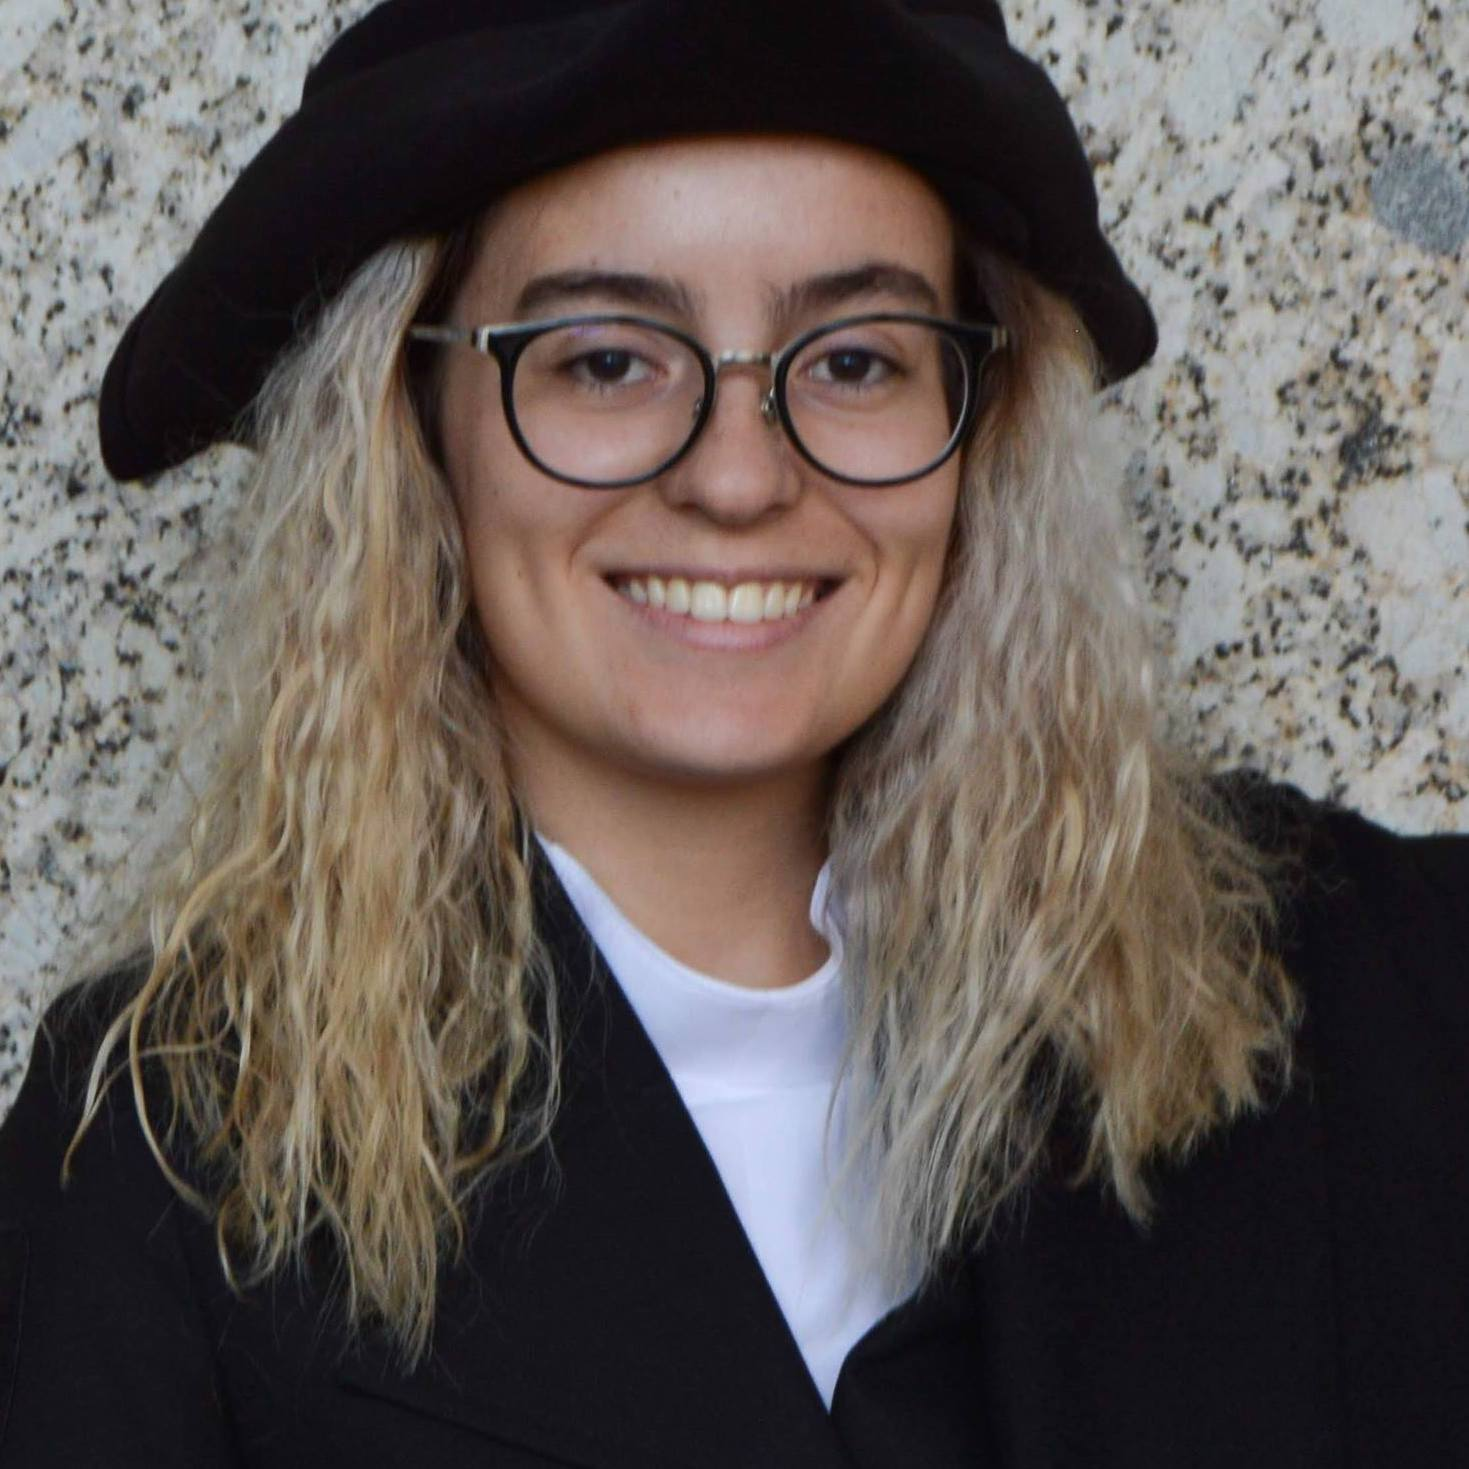
\includegraphics[width=\linewidth]{Pics/86268.jpg}
  \textit{86268 - Maria José Borgpes Pires}
\endminipage\hfill
\minipage{0.32\textwidth}%
  \includegraphics[width=\linewidth]{2.png}
  \textit{numero - nome}
\endminipage
\end{figure}

\vspace{2.0cm}
\text{6 de abril de 2019}

\end{center}
\end{titlepage}

\maketitle

\tableofcontents

\listoffigures


%% Introdução
\chapter{Introdução}

Este trabalho foi desenvolvido no âmbito da unidade curricular laboratórios de informática 3 e tem como objetivo o processamento de dados contidos em 3 ficheiros de texto de modo a responder a queries de forma eficiente, aplicando conhecimentos de algoritmia e programação imperativa.
%% ADICONAR CENAS SOBRE MODULARIDADE
  


%Resolução inicial do problema
\chapter{Resolução inicial do problema}





%% Descrição da Solução Desenvolvida
\chapter{Estruturas de dados}

\chapter{Modularização Funcional e Resolução de queries}











\chapter{Conclusão}





   

\end{document}